\documentclass[12pt,a4paper]{article}

% ─── Page Layout ───────────────────────────────────────────────────────────────
\usepackage[a4paper, margin=0.8in, headheight=14pt]{geometry}

% ─── Fonts (XeLaTeX) ───────────────────────────────────────────────────────────
\usepackage{fontspec}
\usepackage{unicode-math}
\setmainfont{TeX Gyre Pagella}
\setmonofont[Scale=0.88]{TeX Gyre Cursor}
\setmathfont{Latin Modern Math}

% ─── Packages ──────────────────────────────────────────────────────────────────
\usepackage{xcolor}
\usepackage{colortbl}
\usepackage{titlesec}
\usepackage{enumitem}
\usepackage{tabularx}
\usepackage{booktabs}
\usepackage{array}
\usepackage{amsmath}
\usepackage{tikz}
\usetikzlibrary{shapes.geometric, arrows.meta, positioning, calc, fit, decorations.pathreplacing}
\usepackage{tcolorbox}
\tcbuselibrary{skins, breakable}
\usepackage{hyperref}
\usepackage{fancyhdr}
\usepackage{graphicx}
\usepackage{microtype}
\hyphenpenalty=10000
\exhyphenpenalty=10000
\sloppy
\usepackage{caption}
\usepackage{setspace}
\usepackage{multirow}
\usepackage{tocloft}

% ─── Q&A helper ────────────────────────────────────────────────────────────────
\newcommand{\Q}[1]{\textbf{#1}\par\noindent\ignorespaces}

% ─── Colour Palette ────────────────────────────────────────────────────────────
\definecolor{myred}{RGB}{196,30,58}
\definecolor{mydark}{RGB}{30,30,50}
\definecolor{mygreen}{RGB}{14,120,80}
\definecolor{myteal}{RGB}{0,130,140}
\definecolor{myamber}{RGB}{180,100,0}
\definecolor{mypurple}{RGB}{100,30,160}
\definecolor{mygray}{RGB}{246,247,249}
\definecolor{mgframe}{RGB}{180,185,200}
\definecolor{watermark}{RGB}{145,150,170}
\definecolor{hdrred}{RGB}{250,232,235}
\definecolor{hdrgreen}{RGB}{220,244,233}
\definecolor{hdrteal}{RGB}{220,242,244}
\definecolor{hdramber}{RGB}{253,242,215}
\definecolor{hdrpurple}{RGB}{238,228,255}
\definecolor{hdrgray}{RGB}{238,240,245}
\definecolor{rowalt}{RGB}{250,251,253}

% ─── Section Formatting ────────────────────────────────────────────────────────
\titleformat{\section}
  {\large\bfseries\color{myred}}{\thesection.}{0.5em}{}
  [\vspace{1pt}{\color{myred}\rule{\linewidth}{0.8pt}}]
\titleformat{\subsection}
  {\normalsize\bfseries\color{myteal}}{\thesubsection}{0.5em}{}
\titlespacing*{\section}{0pt}{18pt}{7pt}
\titlespacing*{\subsection}{0pt}{11pt}{4pt}

% ─── Paragraph ─────────────────────────────────────────────────────────────────
\setlength{\parindent}{0pt}
\setlength{\parskip}{4pt}

% ─── TOC Styling ───────────────────────────────────────────────────────────────
\renewcommand{\cfttoctitlefont}{\large\bfseries\color{myred}}
\renewcommand{\cftaftertoctitle}{\par\noindent{\color{myred}\rule{\linewidth}{0.8pt}}}
\setlength{\cftbeforetoctitleskip}{0pt}
\setlength{\cftaftertoctitleskip}{6pt}
\renewcommand{\cftsecfont}{\normalsize\bfseries\color{mydark}}
\renewcommand{\cftsecpagefont}{\normalsize\bfseries\color{mydark}}
\renewcommand{\cftsecleader}{\cftdotfill{\cftdotsep}}
\setlength{\cftbeforesecskip}{7pt}
\renewcommand{\cftsubsecfont}{\small\color{mydark}}
\renewcommand{\cftsubsecpagefont}{\small\color{mydark}}
\setlength{\cftbeforesubsecskip}{3pt}
\setlength{\cftsubsecindent}{1.4em}

% ─── Table helpers ─────────────────────────────────────────────────────────────
\renewcommand{\arraystretch}{1.45}
\setlength{\tabcolsep}{6pt}
\arrayrulecolor{mydark}
\newcolumntype{B}[1]{>{\small\bfseries\raggedright\arraybackslash}m{#1}}
\newcolumntype{Y}{>{\small\raggedright\arraybackslash}X}
\renewcommand{\tabularxcolumn}[1]{m{#1}}

% ─── Header / Footer ───────────────────────────────────────────────────────────
\pagestyle{fancy}
\fancyhf{}
\fancyhead[L]{\small\color{myred}\textbf{PE-EC701A}\;\color{mydark}--- Microwave Theory and Technique}
\fancyhead[R]{\small\color{myteal}\textbf{Module 8 Notes}}
\fancyfoot[C]{\small\color{mydark}\thepage}
\fancyfoot[R]{\small\color{watermark}\textit{\copyright\ Biraj}}
\renewcommand{\headrulewidth}{0.5pt}
\renewcommand{\footrulewidth}{0.3pt}

% ─── Hyperref ──────────────────────────────────────────────────────────────────
\hypersetup{
  colorlinks=true, linkcolor=myteal, urlcolor=myteal,
  pdfauthor={Biraj Sarkar},
  pdftitle={PE-EC701A --- Module 8 Notes}
}

% ─── tcolorbox styles ──────────────────────────────────────────────────────────
\tcbset{
  tikzbox/.style={
    colback=mygray, colframe=mgframe, boxrule=0.6pt, arc=4pt,
    left=8pt, right=8pt, top=6pt, bottom=6pt,
    colbacktitle=mgframe, coltitle=mydark,
    fonttitle=\small\bfseries
  },
  defbox/.style={
    colback=hdrgreen, colframe=mygreen, boxrule=0.8pt, arc=4pt,
    left=9pt, right=9pt, top=6pt, bottom=6pt,
    colbacktitle=mygreen, coltitle=white,
    fonttitle=\small\bfseries
  },
  formulabox/.style={
    colback=hdrteal, colframe=myteal, boxrule=0.8pt, arc=4pt,
    left=9pt, right=9pt, top=7pt, bottom=7pt,
    colbacktitle=myteal, coltitle=white,
    fonttitle=\small\bfseries
  },
  examplebox/.style={
    colback=hdramber, colframe=myamber, boxrule=0.8pt, arc=4pt,
    left=9pt, right=9pt, top=6pt, bottom=6pt,
    colbacktitle=myamber, coltitle=white,
    fonttitle=\small\bfseries
  },
  masonbox/.style={
    colback=hdrpurple, colframe=mypurple, boxrule=0.8pt, arc=4pt,
    left=9pt, right=9pt, top=6pt, bottom=6pt,
    colbacktitle=mypurple, coltitle=white,
    fonttitle=\small\bfseries
  },
  exambox/.style={
    colback=hdrpurple, colframe=mypurple, boxrule=1pt, arc=5pt,
    left=10pt, right=10pt, top=8pt, bottom=8pt,
    colbacktitle=mypurple, coltitle=white,
    fonttitle=\bfseries,
    breakable, title after break={\textbf{Frequently Asked / Viva Questions (contd.)}}}
}
% Make all boxes breakable across pages
\tcbset{breakable}

% ─── TikZ styles ───────────────────────────────────────────────────────────────
\tikzset{
  block/.style={rectangle, draw=myteal, fill=hdrteal,
    text width=2.4cm, align=center, minimum height=0.95cm,
    font=\small, rounded corners=3pt, line width=0.7pt},
  redblock/.style={rectangle, draw=myred, fill=hdrred,
    text width=2.4cm, align=center, minimum height=0.95cm,
    font=\small, rounded corners=3pt, line width=0.7pt},
  netnode/.style={rectangle, draw=myteal, fill=hdrteal,
    text width=1.5cm, align=center, minimum height=0.8cm,
    font=\small, rounded corners=3pt, line width=0.7pt},
  sumjunc/.style={circle, draw=myamber, fill=hdramber,
    minimum size=0.62cm, font=\small, line width=0.8pt},
  snode/.style={circle, draw=mypurple, fill=hdrpurple,
    minimum size=0.55cm, font=\footnotesize, line width=0.7pt},
  arrow/.style={-Stealth, thick, color=mydark},
  redarrow/.style={-Stealth, thick, color=myred},
  line/.style={thick, color=mydark}
}

% ═══════════════════════════════════════════════════════════════════════════════
\begin{document}
% ═══════════════════════════════════════════════════════════════════════════════

\begin{center}
  {\LARGE\bfseries\color{myred} PE-EC701A --- Microwave Theory and Technique}\\[5pt]
  {\normalsize\color{mydark} Semester VII \quad$\bullet$\quad 3L:0T:0P \quad$\bullet$\quad 3 Credits}\\[3pt]
  {\normalsize\color{myteal}\textbf{Module 8 Exam Notes: Microwave Measurements}}\\[3pt]
  {\small\color{mydark} CGEC \;$|$\; B.Tech ECE (2023--27) \;$|$\; \textit{Biraj Sarkar}}
\end{center}
\vspace{2pt}
\noindent{\color{myred}\rule{\linewidth}{1.5pt}}
\vspace{2pt}

\hypersetup{linkcolor=mydark}
\tableofcontents
\hypersetup{linkcolor=myteal}
\newpage

% ===============================================================================
\section{Power Measurement}
% ===============================================================================

Microwave power is categorized based on intensity levels: Low Power ($< 10$ mW), Medium Power (10 mW -- 10 W), and High Power ($> 10$ W).

\subsection{Bolometer Mount Method (Low Power)}
A bolometer is a temperature-sensitive resistor whose resistance changes when it absorbs RF power.
\begin{itemize}[leftmargin=*, itemsep=3pt]
  \item \textbf{Thermistor:} Has a \textbf{negative temperature coefficient (NTC)}; resistance decreases as temperature rises.
  \item \textbf{Barretter:} Has a \textbf{positive temperature coefficient (PTC)}; resistance increases as temperature rises.
\end{itemize}
The bolometer is placed in an active arm of a self-balancing Wheatstone bridge. The DC bias power required to balance the bridge is measured before and after applying RF power:
\begin{equation}
  P_{\text{RF}} = P_{\text{bias,1}} - P_{\text{bias,2}}
\end{equation}

\subsection{Calorimetric Method (High Power)}
High power is measured by absorbing the RF energy in a fluid load (usually water) and measuring the temperature rise ($\Delta T = T_{\text{out}} - T_{\text{in}}$).
\begin{equation}
  P_{\text{RF}} = \dot{m} C_p \Delta T
\end{equation}
where $\dot{m}$ is mass flow rate and $C_p$ is specific heat.

% ===============================================================================
\section{Impedance and Frequency Measurement}
% ===============================================================================

\subsection{Slotted Line Probe Technique}
A slotted line is a section of coaxial line or waveguide containing an axial slot that allows a small capacitive probe to slide along the length to sample the electric field.

\begin{tcolorbox}[tikzbox, title={Slotted Line Probe Mechanism}]
\centering
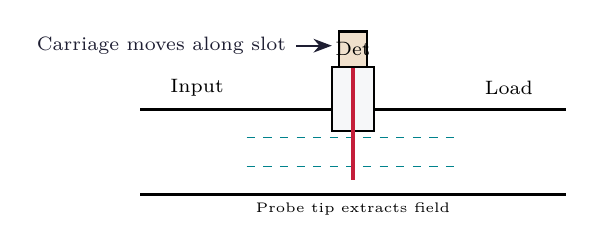
\begin{tikzpicture}[scale=0.9, every node/.style={font=\scriptsize}]
  % Waveguide segment
  \draw[very thick] (0,0.6) -- (6,0.6);
  \draw[very thick] (0,-0.6) -- (6,-0.6);
  
  % Slot representation (dashed lines)
  \draw[dashed, color=myteal] (1.5,0.2) -- (4.5,0.2);
  \draw[dashed, color=myteal] (1.5,-0.2) -- (4.5,-0.2);
  
  % Slide probe carriage
  \draw[thick, fill=mygray] (2.7,0.3) rectangle (3.3,1.2);
  \draw[line width=1.5pt, color=myred] (3.0, 1.2) -- (3.0, -0.4); % Probe tip
  
  % Crystal detector block on top
  \draw[thick, fill=myamber!20] (2.8,1.2) rectangle (3.2,1.7) node[midway] {Det};
  
  \node at (0.8,0.9) {Input};
  \node at (5.2,0.9) {Load};
  \node[font=\tiny] at (3.0, -0.8) {Probe tip extracts field};
  \draw[arrow] (2.2, 1.5) node[left] {Carriage moves along slot} -- (2.7, 1.5);
\end{tikzpicture}
\end{tcolorbox}

\begin{itemize}[leftmargin=*, itemsep=3pt]
  \item \textbf{Low VSWR Measurement ($1 < S < 10$):} Measured directly as the ratio of maximum to minimum probe outputs:
    \begin{equation}
      S = \frac{V_{\text{max}}}{V_{\text{min}}}
    \end{equation}
  \item \textbf{High VSWR Measurement (Double-Minimum Method, $S > 10$):}
    For high reflection, the minimum is sharp and close to the noise floor. We measure the distance $\Delta x$ between two positions where output power is twice the minimum value:
    \begin{equation}
      S = \frac{\lambda_g}{\pi \Delta x}
    \end{equation}
\end{itemize}

% ===============================================================================
\section{Vector Network Analyzer (VNA)}
% ===============================================================================

A Vector Network Analyzer measures the complete S-parameters (both magnitude and phase) of a device under test (DUT) by separating incident, reflected, and transmitted waves.

\begin{tcolorbox}[tikzbox, title={Vector Network Analyzer Simplified Architecture}]
\centering
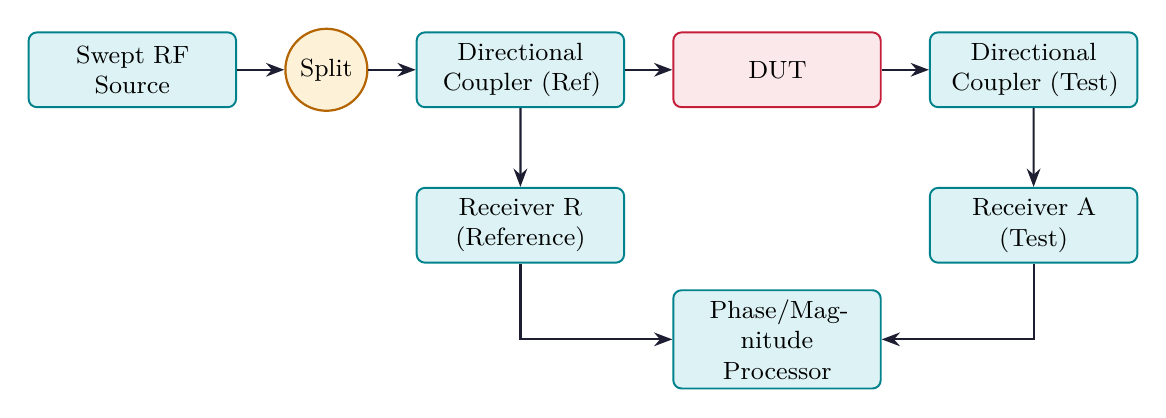
\begin{tikzpicture}[scale=0.9, every node/.style={font=\scriptsize}]
  \node[block] (src) {Swept RF\\Source};
  \node[sumjunc, right=0.6cm of src] (div) {Split};
  \node[block, right=0.6cm of div] (coup1) {Directional\\Coupler (Ref)};
  \node[block, right=0.6cm of coup1, draw=myred, fill=hdrred] (dut) {DUT};
  \node[block, right=0.6cm of dut] (coup2) {Directional\\Coupler (Test)};
  
  \node[block, below=1.0cm of coup1] (rec1) {Receiver R\\(Reference)};
  \node[block, below=1.0cm of coup2] (rec2) {Receiver A\\(Test)};
  
  \node[block, below=2.3cm of dut] (dsp) {Phase/Magnitude\\Processor};
  
  \draw[arrow] (src) -- (div);
  \draw[arrow] (div) -- (coup1);
  \draw[arrow] (coup1) -- (dut);
  \draw[arrow] (dut) -- (coup2);
  
  \draw[arrow] (coup1) -- (rec1);
  \draw[arrow] (coup2) -- (rec2);
  
  \draw[arrow] (rec1.south) |- (dsp.west);
  \draw[arrow] (rec2.south) |- (dsp.east);
\end{tikzpicture}
\end{tcolorbox}

\textbf{Calibration:} System errors are calibrated out using the \textbf{SOLT} (Short, Open, Load, Thru) standard calibration procedure.

% ===============================================================================
\section{Spectrum Analyzer}
% ===============================================================================

A Spectrum Analyzer displays signal amplitude versus frequency, identifying harmonics, distortion, and noise floors.

\begin{tcolorbox}[tikzbox, title={Superheterodyne Spectrum Analyzer Block Diagram}]
\centering
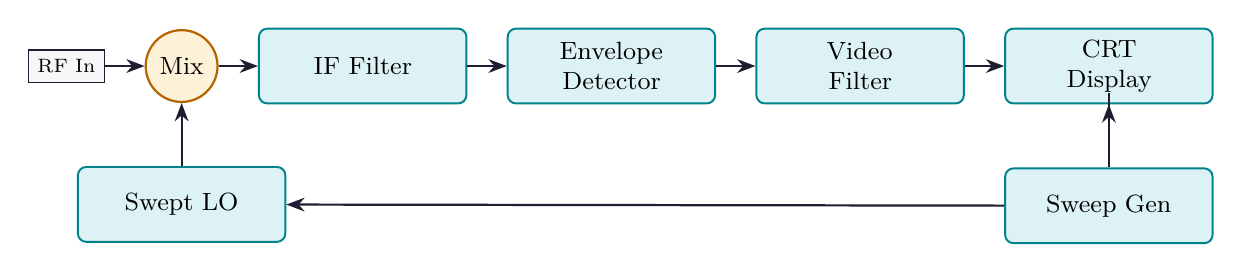
\begin{tikzpicture}[node distance=0.2cm and 0.5cm, every node/.style={font=\scriptsize}]
  \node[draw=mydark, fill=mygray, minimum size=0.4cm] (in) {RF In};
  \node[sumjunc, right=0.5cm of in] (mix) {Mix};
  \node[block, right=0.5cm of mix] (if) {IF Filter};
  \node[block, right=0.5cm of if] (det) {Envelope\\Detector};
  \node[block, right=0.5cm of det] (vid) {Video\\Filter};
  \node[block, right=0.5cm of vid] (crt) {CRT\\Display};
  
  \node[block, below=0.8cm of mix] (lo) {Swept LO};
  \node[block, below=0.8cm of crt] (swp) {Sweep Gen};
  
  \draw[arrow] (in) -- (mix);
  \draw[arrow] (mix) -- (if);
  \draw[arrow] (if) -- (det);
  \draw[arrow] (det) -- (vid);
  \draw[arrow] (vid) -- (crt);
  \draw[arrow] (lo) -- (mix);
  \draw[arrow] (swp) -- (lo);
  \draw[arrow] (swp) |- (crt.south);
\end{tikzpicture}
\end{tcolorbox}

% ===============================================================================
\section{Noise Measurement: Y-Factor Method}
% ===============================================================================

The Y-factor method is the standard technique for measuring the noise figure ($F$) of a receiver:

\begin{tcolorbox}[formulabox, title={\textbf{Y-Factor Method Equations}}]
We measure output noise power with a hot noise source at temperature $T_h$ and a cold noise source at temperature $T_c$. The ratio is:
\begin{equation}
  Y = \frac{N_{\text{hot}}}{N_{\text{cold}}} = \frac{T_h + T_e}{T_c + T_e}
\end{equation}
Solving for the equivalent noise temperature $T_e$ of the receiver:
\begin{equation}
  T_e = \frac{T_h - Y T_c}{Y - 1} \quad (\text{K})
\end{equation}
The noise figure $F$ is then calculated as:
\begin{equation}
  F = 1 + \frac{T_e}{T_0} \quad (\text{with } T_0 = 290\text{ K})
\end{equation}
\end{tcolorbox}

% ===============================================================================
% MANDATORY QUICK REVISION PAGE
% ===============================================================================
\newpage
\begin{center}
  {\large\bfseries\color{myred} Quick Revision --- Module VIII}\\[3pt]
  {\small\color{mydark} Microwave Measurements $|$ PE-EC701A}
\end{center}
\noindent{\color{myred}\rule{\linewidth}{1.2pt}}
\vspace{4pt}

\begin{tcolorbox}[formulabox, title={\textbf{Key Formulas at a Glance}}]
\renewcommand{\arraystretch}{1.3}
\begin{tabularx}{\linewidth}{B{4.5cm} X}
Low VSWR                & $S = \frac{V_{\text{max}}}{V_{\text{min}}}$ \\[4pt]
Double-Minimum VSWR     & $S = \frac{\lambda_g}{\pi \Delta x}$ \quad ($\Delta x$ is distance between $2V_{\text{min}}$ points) \\[4pt]
Calorimetric Power      & $P = \dot{m} C_p (T_{\text{out}} - T_{\text{in}})$ \\[4pt]
Y-Factor Relation       & $Y = \frac{N_{\text{hot}}}{N_{\text{cold}}} = \frac{T_h+T_e}{T_c+T_e}$ \\[4pt]
Receiver Noise Temp     & $T_e = \frac{T_h - Y T_c}{Y - 1}$
\end{tabularx}
\tcbset{colbacktitle=mygreen, coltitle=white}
\end{tcolorbox}

\begin{tcolorbox}[defbox, title={\textbf{One-Line Definitions}}]
\begin{itemize}[leftmargin=*, itemsep=2.5pt, topsep=0pt]
  \item \textbf{Thermistor:} A temperature-sensitive resistor with a negative temperature coefficient (NTC).
  \item \textbf{Barretter:} A thin platinum wire bolometer element with a positive temperature coefficient (PTC).
  \item \textbf{Slotted Line:} A waveguide with an axial slot used to sample electric field standing wave patterns.
  \item \textbf{VNA:} An instrument that measures the amplitude and phase of reflection/transmission S-parameters.
  \item \textbf{Spectrum Analyzer:} A swept receiver displaying power spectral density versus frequency.
  \item \textbf{Y-Factor:} The ratio of receiver output noise powers under hot and cold source excitations.
  \item \textbf{SOLT Calibration:} Standard VNA calibration using Short, Open, Load, and Thru reference elements.
\end{itemize}
\end{tcolorbox}

\begin{tcolorbox}[exambox, title={\textbf{Frequently Asked / Viva Questions}}]
\begin{enumerate}[topsep=0pt, label=\textbf{Q\arabic*.}, itemsep=5pt]
  \item \Q{Explain why a bolometer Wheatstone bridge must be self-balancing.}
    Applying RF power heats the bolometer, changing its resistance and unbalancing the bridge. Automatically reducing DC bias to re-balance the bridge allows RF power to be measured from the DC power difference, keeping bolometer resistance constant.
  \item \Q{What is the double-minimum method and when is it used?}
    It is a method to measure high VSWR ($S > 10$). We measure the distance $\Delta x$ between the $3\text{ dB}$ points around a standing-wave minimum. It is used because direct $V_{\text{max}}/V_{\text{min}}$ measurements are inaccurate near the noise floor.
  \item \Q{What is the difference between a scalar and a vector network analyzer?}
    A Scalar Network Analyzer (SNA) only measures amplitude transmission and reflection coefficients. A Vector Network Analyzer (VNA) measures both amplitude and phase.
  \item \Q{Why does a frequency wavemeter have a resonant cavity?}
    It is a tunable cavity resonator. When tuned to the input frequency, it absorbs a fraction of power, creating a dip in the through-line power meter to indicate frequency.
  \item \Q{Explain the SOLT calibration method.}
    VNA calibration standards: Short circuit (reflects phase $180^\circ$), Open circuit (reflects phase $0^\circ$), matched Load (absorbs all power), and Thru connection (connects ports directly).
  \item \Q{Describe the basic block diagram of a superheterodyne spectrum analyzer.}
    RF input is mixed with a swept LO. The resulting IF signal is filtered, envelope-detected, and displayed on a screen swept in sync with the LO.
  \item \Q{How is antenna gain measured using the comparison method?}
    The received power of a standard gain horn (known gain $G_s$) is measured. The test antenna is then substituted, and its received power $P_t$ is measured. The test gain is $G_t = G_s (P_t/P_s)$.
  \item \Q{Why is calorimetric power measurement used for high powers?}
    Because solid-state sensors (bolometers/diodes) saturate or burn out at high powers. Fluid loads can absorb kilowatts of power safely, converting it to measurable heat.
  \item \Q{What is the physical meaning of the equivalent noise temperature ($T_e$)?}
    It is the temperature of a dummy resistor at the input of an ideal noiseless receiver that would generate the same noise power as the actual noisy receiver.
  \item \Q{Why is the slot in a slotted line waveguide cut along the center of the broad wall?}
    Because the slot is parallel to the surface current flow lines of the dominant $\text{TE}_{10}$ mode. This minimizes field distortion and leakage.
  \item \Q{What are the typical noise sources used in Y-factor measurements?}
    Gas discharge tubes or avalanche diodes that can switch between a room temperature state (cold) and a high electron temperature state (hot).
  \item \Q{How does a Spectrum Analyzer differ from an Oscilloscope?}
    An oscilloscope displays signal amplitude versus time (time domain). A spectrum analyzer displays signal amplitude versus frequency (frequency domain).
\end{enumerate}
\tcbset{colbacktitle=mgframe, coltitle=mydark}
\end{tcolorbox}

\begin{tcolorbox}[tikzbox, title={Comparison of VNA and Spectrum Analyzer}]
\renewcommand{\arraystretch}{1.4}
\par\noindent
\begin{tabularx}{\linewidth}{|B{3.0cm}|Y|Y|}
\hline
\rowcolor{hdrgray}
\textbf{Feature} & \textbf{Vector Network Analyzer (VNA)} & \textbf{Spectrum Analyzer} \\
\hline
\textbf{Signal Source} & Built-in swept source (active stimulus). & None (passive measurement of external signal). \\
\hline
\rowcolor{rowalt}
\textbf{Quantities Measured} & S-parameters ($S_{11}, S_{21}$, etc.), phase, group delay. & Frequency component amplitudes, harmonics, noise floor. \\
\hline
\textbf{Calibration} & Extremely complex (SOLT calibration required). & Simple amplitude calibration. \\
\hline
\rowcolor{rowalt}
\textbf{Primary Use} & Characterizing passive/active components (filters, antennas). & Analyzing transmitter signals, interference, distortion. \\
\hline
\end{tabularx}
\end{tcolorbox}

\end{document}
